%------------------------------------------------------------------------------------------
% PACKAGES AND OTHExsssR DOCUMEffdfdNT CONFIGURATIONS
%------------------------------------------------------------------------------------------
\documentclass[12pt]{article}
\usepackage{mathpazo}
%\usepackage{merriweather}
%\usepackage{libertine}
%\usepackage{libertinust1math}
%\usepackage[defaultsans]{droidsans}
%\renewcommand*\familydefault{\sfdefault}
%\usepackage[sfdefault,condensed]{roboto}
%\usepackage{cmbright}
%\usepackage[default,osfigures,scale=0.95]{opensans}
%\usepackage{tgpagella}
\usepackage[a4paper, total={6.2in, 9in}]{geometry}
\usepackage{url}
\usepackage{graphics}
\usepackage{graphicx}
\usepackage[T1]{fontenc}
\usepackage{amsmath}

\usepackage[pdftex]{hyperref}
%\usepackage[symbol]{footmisc}
\linespread{1.05}
\hypersetup{
   backref=section,
   bookmarksopen=true,
   bookmarksnumbered=true,
   bookmarksopenlevel=2,
   pdftitle={Master Thesis Proposal},
   pdfauthor={Mohammed Shameer Abubucker <mohammed.abubucker@smail.inf.h-brs.de>},
   pdfkeywords= {motion planning, humanoids, HRP4},
   %citecolor=blue,
   %citebordercolor={0 0.4 0.7}
   colorlinks,
   citecolor=blue,
   filecolor=black,
   linkcolor=black,
   urlcolor=black
}
\newcommand{\myspace}{\\\\}
\newcommand{\HRule}{\rule{\linewidth}{0.6mm}} 
\begin{document}
\begin{titlepage}

% Defines vjhvjva new command for
% the horizontal lines, change thickness here

\center % Center everything on thecf page
 
%----------------------------------------------------------------------------------------
%	HEADING SECTIONS
%----------------------------------------------------------------------------------------

\Large{Master Thesis Proposal}\\[1.5cm] 
%----------------------------------------------------------------------------------------
%	TITLE SECTION
%----------------------------------------------------------------------------------------
\HRule
% \HRule \\[0.4cm]
{ \Large \bfseries Learning High-Level Environment Dynamics}\\\HRule \\[0.4cm]
% Title of your document
% \HRule
% \\[1.5cm]

\vspace*{1.5\baselineskip}
 
\normalsize{\bfseries Kaviya Dhanabalachandran
\footnote{\href{kaviya.dhanabalachandran@smail.inf.h-brs.de}{kaviya.dhanabalachandran@smail.inf.h-brs.de}}}\\[0.25cm]
% Minor heading such as course title
{\normalsize Master of Autonomous Systems}\\[0.5cm] % Minor heading such as
% course title
{\small Bonn-Rhein-Sieg University of Applied Sciences, Sankt
Augustin, Germany.}\\[0.05cm]
\&
\\[0.05cm]
% Minor heading such as course title
{\small Robert Bosch GmbH,\\ Robert-Bosch-Campus 1, 71272,\\ Renningen, Germany.}\\[0.7cm]
\small{\today}\\[1,5cm]
%April 24th, 2015
%----------------------------------------------------------------------------------------
%	AUTHOR SECTION
%----------------------------------------------------------------------------------------
%\vspace*{6\baselineskip} % Whitespace between location/year and editors


%\end{minipage}

\end{titlepage}
%%%%%%%%
%%%%%%%
\section{Introduction}
\begin{itemize}
\item With growing demand for personal robots that could assist the elderly, perform the daily repetitive tasks in households and offices, there is a persistent need to develop robots that could operate autonomously over a long period of time.
\item There are a number of challenges to overcome, to develop and maintain a robot that can perform tasks in a dynamic unstructured environment and co-exist with human beings.
\item One of the problems of working in a dynamic unstructured environment is the robot has to foresee all possible circumstances it has to handle.  
\item A robot which operate over a long time should have the capability to learn from its experience, to be robust.
\\
\item Navigation is one of the essential ability for a personal robot to do the tasks and interact with an environment. 
\item We focus on the problem of improving navigation in a dynamic environment. 
\item Traditionally, a map which is created once after exploring in the environment is used for navigation. Any discrepancies from the initially created map is considered as sensor noise.
\item Dynamic changes are not taken into account for constructing a map. 
\item A robot has to replan whenever there was a moving obstacle.
\item In this project, we try to learn the dynamic changes over time to improve navigation in indoor environment.
\end{itemize}
%%%%%%%
%%%%%%%
\section{Related Work}

%%%%%%%
%%%%%%%
\section{Problem Formulation}

%%%%%%%
%%%%%%%
\section{Approach}\label{sec:approach}


\section{Deliverables}
\begin{itemize} 
\item \textbf{Minimum}

\item \textbf{Expected}
 

\item \textbf{Maximum}

\end{itemize}

\section{Work Plan}

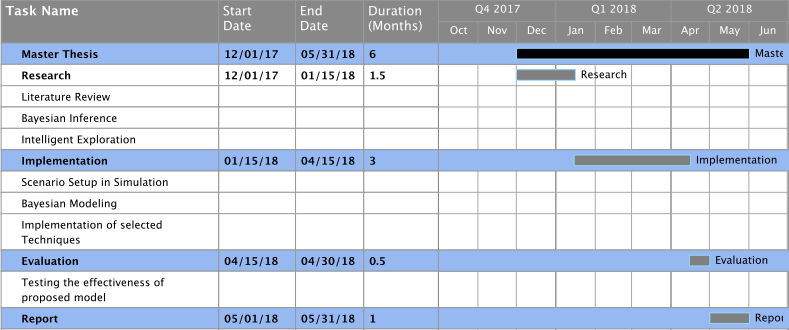
\includegraphics[width=\textwidth, height=6cm]{workplan.png}

%%%%%%%
\vspace*{6\baselineskip}
\newpage
\bibliography{thesis_proposal}
\bibliographystyle{unsrt}

\end{document}